\tikzstyle{tag} = [minimum height=1.5em, minimum width=1.5em]
\tikzstyle{letter} = [draw, thin, fill=blue!20, minimum height=1.5em, minimum width=1.5em]
\tikzstyle{module} = [rectangle, draw, thin, fill=green!20, minimum height=1.5em]
\tikzstyle{module-1} = [module, minimum width=1.5em]
\tikzstyle{module-2} = [module, minimum width=6.7em]
\tikzstyle{module-3} = [module, minimum width=22.3em]
    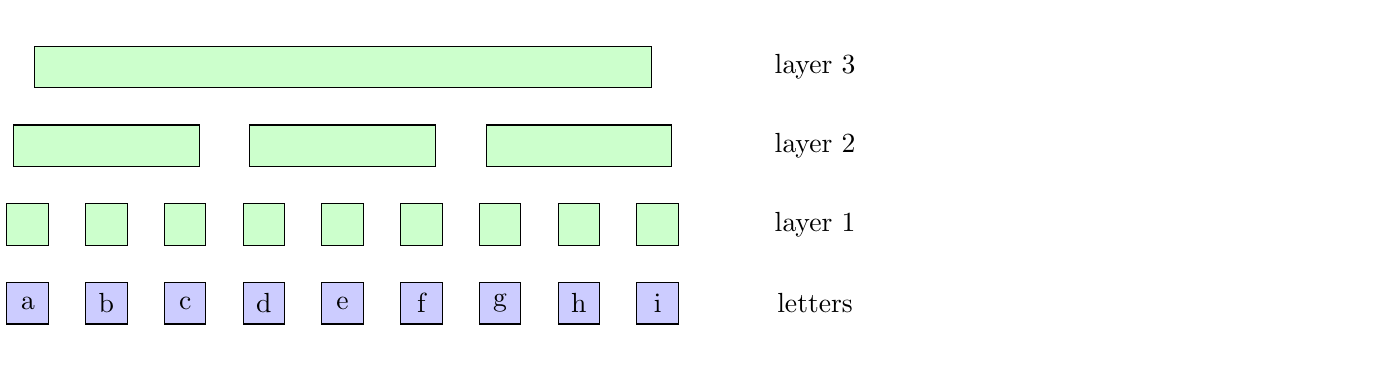
\begin{tikzpicture}
      \path[use as bounding box] (0,-0.5) rectangle (17,3.5);
      
      \path[->] node[letter] (a) at (0,0) {a};
      \path[->] node[letter] (b) at (1,0) {b};
      \path[->] node[letter] (c) at (2,0) {c};
      \path[->] node[letter] (d) at (3,0) {d};
      \path[->] node[letter] (e) at (4,0) {e};
      \path[->] node[letter] (f) at (5,0) {f};
      \path[->] node[letter] (g) at (6,0) {g};
      \path[->] node[letter] (h) at (7,0) {h};
      \path[->] node[letter] (i) at (8,0) {i};
      
      \path[->] node[tag] (letters) at (10,0) {letters};
      
      \path[->] node[module-1] (m-a) at (0,1) {};
      \path[->] node[module-1] (m-b) at (1,1) {};
      \path[->] node[module-1] (m-c) at (2,1) {};
      \path[->] node[module-1] (m-d) at (3,1) {};
      \path[->] node[module-1] (m-e) at (4,1) {};
      \path[->] node[module-1] (m-f) at (5,1) {};
      \path[->] node[module-1] (m-g) at (6,1) {};
      \path[->] node[module-1] (m-h) at (7,1) {};
      \path[->] node[module-1] (m-i) at (8,1) {};
      
      \path[->] node[tag] (layer1) at (10,1) {layer 1};
      
      \path[->] node[module-2] (m-abc) at (1,2) {};
      \path[->] node[module-2] (m-def) at (4,2) {};
      \path[->] node[module-2] (m-ghi) at (7,2) {};
      
      \path[->] node[tag] (layer2) at (10,2) {layer 2};
      
      \path[->] node[module-3] (m-ghi) at (4,3) {};
      
      \path[->] node[tag] (layer3) at (10,3) {layer 3};
    \end{tikzpicture}